\chapter{Automatisation du processus d'investigation}
\label{Automatisation du processus d'investigation}
\thispagestyle{fancy}
Lorsqu'une error name est révélée (partie \ref{Introduction:Expression du besoin:Hiérarchisation des erreurs}) durant le Filtering test, de nombreuses données sont enregistrées dans un fichier journal (que l'on retrouve plus souvent sous le terme anglais de fichier "log".) Une analyse poussée de ces informations permet de déterminer la root cause liée à l'error name (partie \ref{Introduction:Expression du besoin:Hiérarchisation des erreurs}). Afin d'automatiser ce processus d'analyse, on s'appuie sur l'utilisation d'algorithmes d'apprentissage automatique. 

\section{Architecture High Level du système proposé}
\label{Automatisation du processus d'investigation: Achitecture High Level du système proposé}
L'architecture haut niveau de la solution que l'on propose est composée de deux couches: une couche "root cause" et une couche "error name".
\begin{description}
	\item [Couche root cause] La couche root cause permet de détecter la présence d'une root cause dans l'exemple que l'on analyse. Il s'agit d'un algorithme d'apprentissage automatique entraîné à effectuer cette tâche.
	\item [Couche error name] La couche error name est constituée d'un ensemble de couches root cause de telle manière que lorsqu'un fichier historique est mis en entrée du système, l'ensemble des couches root cause sont activées. Ainsi, le système recherche la présence de chaque root cause connue dans l'exemple étudié. On obtient en sortie de la couche error name le nom de la root cause ayant la plus forte probabilité d'avoir été reconnue.
\end{description} 

\subsubsection{Exemple de mise en place  d'une couche error name et de ses couches root cause}
Afin d'exposer de manière concrète le fonctionnement de l'architecture haut niveau de la solution proposée, on soumet un exemple de mise en place d'une architecture de détection et son utilisation . \\

\paragraph{Mise en place du système de détection d'une root cause / Apprentissage}
On souhaite dans un premier temps mettre en place l'architecture permettant de détecter la cause (root cause) ayant entrainé la chute du robot lors du Filtering test (error name). Cette étape consiste à créer les couches root cause, i.e. entrainer différents algorithmes d'apprentissage automatique à reconnaitre la root cause pour laquelle ils ont été crée (figure \ref{fig:Creation des couches root cause}). Afin d'entraîner ces couches, on utilise les données utiles à chaque root cause, contenues dans le fichier log généré lors de la chute d'un robot durant du Filtering Test. Par exemple, dans le cas de la root cause "frottement des freins de la hanche", on utilisera les données "valeurs du senseur de la hanche" et "valeurs de l'actuateur de la hanche". Ces deux éléments correspondre aux features de notre apprentissage (c.f. partie \ref{Le Machine Learning: Généralités sur le Machine Learning: Définition et principe général:Lexique}). L'ensemble de ces couches root cause sont placées dans la couche error name associée. Ici, il s'agit de la couche permettant de déterminer la cause de la chute d'un robot.

\begin{figure}[h]
	\centering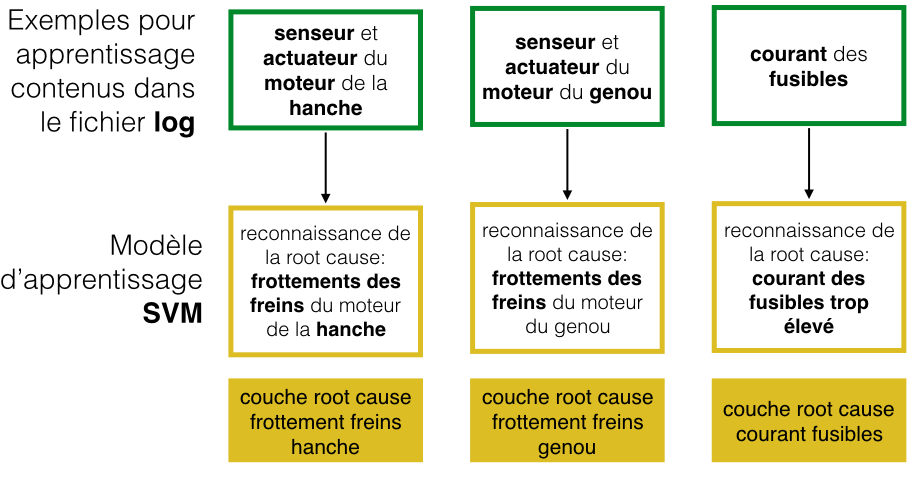
\includegraphics[height=7.5cm]{images/synoptique_root.png}
	\caption[Creation des couches root cause]{Synoptique haut niveau de la création des couches root cause. Les couches root cause correspondent à des algorithmes d'apprentissage automatique que l'ont entraîne à détecter la root cause à laquelle ils sont associés. Par exemple, créer la couche root cause "frottement du frein de la hanche" revient à entraîner un algorithme d'apprentissage de type SVM à partir des valeurs senseurs et actuateurs de la hanches contenues dans les différents exemples de fichiers logs générés lors de chutes de robot durant le filtering test. On réalise ce processus pour chaque couche root cause que l'on veut créer.}
	\label{fig:Creation des couches root cause}
\end{figure}

\paragraph{Utilisation du système de détection d'une root cause}
Une fois nos différentes couches root cause crées, on souhaite utiliser notre système afin de détecter la cause de la chute d'un robot (c.f. figure \ref{fig:utilisation de la couche error name}). Pour cela, on place à l'entrée de notre couche error name le fichier log que l'on souhaite analyser. Chaque couche root cause extrait du fichier log les features qui lui sont liées (e.g. la root cause "frottement des freins de la hanche" est liée aux features senseurs et actuateurs de la hanche). L'algorithme SVM de chaque couche root cause va alors émettre une décision quant à la présence ou non de la root cause dans le fichier log; Cette décision correspond à la probabilité que la root cause ai été détecté (en \%). La couche root cause ayant la probabilité la plus élevé en sortie est considéré comme la root cause (cause) ayant entrainé l'error name (i.e. la conséquence, ici la chute du robot) 

\begin{figure}[h]
	\centering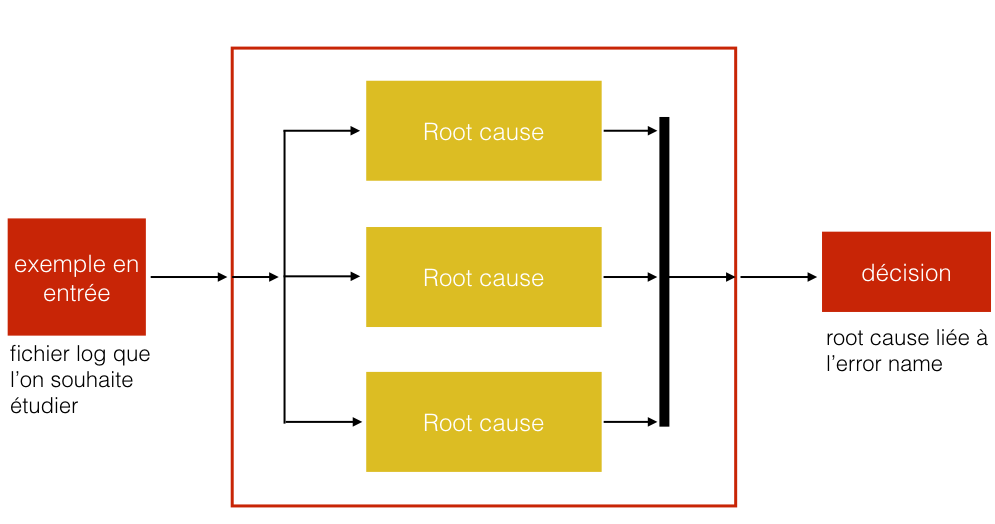
\includegraphics[height=8.5cm]{images/synoptique_error.png}
	\caption[Utilisation de la couche error name]{Synoptique haut niveau de l'utilisation de la couche error name. La couche error name contient plusieurs couches root cause. On met en entrée du système le fichier log que l'on souhaite analyser, puis chaque couche root cause va détecter la présence de la root cause à laquelle elle est rattachée. On obtient en sortie de la couche error name la root cause  ayant la plus forte probabilité d'avoir été reconnue.}
	\label{fig:utilisation de la couche error name}
\end{figure}

Chaque couche root cause peut être considérée comme un système à part entière. Le schéma fonctionnel d'une root cause (c.f. figure 	\ref{fig:Synoptique d'une couche root cause}) reprend la même structure que celui du Machine Learning (c.f. \ref{fig:Schéma fonctionnel haut niveau du Machine Learning}) car, comme dit précédemment, chaque root cause est constitué d'un instance de l'algorithme SVM. Dans la suite de notre étude de l'architecture haut niveau de la solution proposée, on s'intéressera plus particulièrement  au fonctionnement de la couche root cause car elle contient l'ensemble du traitement et de l'analyse des données.

\begin{figure}[h]
	\centering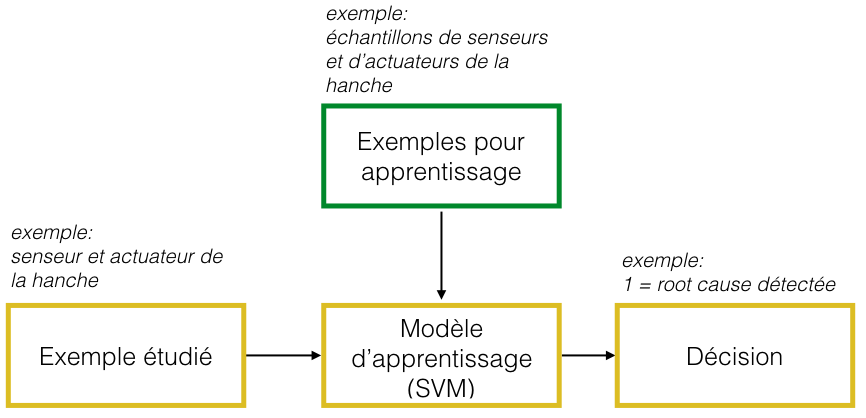
\includegraphics[height=7.4cm]{images/exemple_root.png}
	\caption[Synoptique d'une couche root cause]{Synoptique d'une couche root cause. La couche error name contient plusieurs couches root cause. On met en entrée du système le fichier log que l'on souhaite analyser, puis chaque couche root cause va détecter la présence de la root cause à laquelle elle est rattachée. On obtient en sortie de la couche error name la root cause  ayant la plus forte probabilité d'avoir été reconnue.}
	\label{fig:Synoptique d'une couche root cause}
\end{figure}

\subsection{Les exemples}
\label{Automatisation du processus d'investigation: Achitecture High Level du système proposé: Les exemples}
Les exemples sont les éléments permettant d'entraîner l'algorithme d'apprentissage automatique (c.f. partie \ref{Le Machine Learning: Généralités sur le Machine Learning: Les données}). Dans le cadre de la résolution de notre problématique, ces exemples correspondent aux données générées et enregistrées dans le fichier log lorsqu'une erreur (error name) est détectée durant le Filtering Test.

\subsection{Structure du fichier log}
\label{Automatisation du processus d'investigation: Achitecture High Level du système proposé: Structure du fichier log}
Le fichier log renferme un ensemble de données enregistrées lors de la détection d'une erreur durant le Filtering Test. Ces données correspondent aux "rythmes vitaux" du robot. Il contient par exemple l'évolution temporelle des différents actuateurs et senseurs de Pepper, la température de différentes pièces mécaniques, etc. Dans le cadre de l'entraînement de l'algorithme du Machine Learning (SVM), chacune de ces constantes correspond à une feature  (c.f. partie  \ref{Le Machine Learning: Généralités sur le Machine Learning: Définition et principe général:Lexique}). Soit le tableau \ref {tab: Extrait du contenu d'un fichier log}, un extrait du contenu d'un fichier log:

\begin{equation}
	\begin{blockarray}{ccccccc}
		\begin{block}{c[cccccc]}
			features & HeadPitchPositionActuatorValue & HeadPitchElectricCurrentSensorValue & HipPitchPositionSensorValue & HipPitchPositionActuatorValue &  KneePitchPositionSensorValue & KneePitchPositionActuatorValue \\
			t_0 & -0,404 & 0,64 & -0,023 & -0,04 & -0,008 & -0,007 \\
			t_1 & -0,404 & 0,64 & -0,029 & -0,038 & -0,006 & -0,006 \\
			t_3 & -0,404 & 0,576 & -0,029 & -0,033 & -0,008 & -0,012 \\
			t_4 & -0,402 & 0,544 & -0,029 & -0,027 & -0,012 & -0,022 \\
			t_5 & -0,401 & 0,448 & -0,029 & -0,027 & -0,015 & -0,029 \\
			t_6 & -0,401 & 0,448 & -0,023 & -0,029 & -0,017 & -0,031 \\
			t_7 & -0,408 & 0,096 & -0,021 & -0,031 & -0,015 & -0,032 \\
			t_8 & -0,444 & 0,096 & -0,021 & -0,032 & -0,015 & 0,035 \\
			t_9 & -0,486 & 0,096 & -0,021 & -0,033 & -0,017 & -0,039 \\
			t_{10} & -0,523 & 0,128 & -0,021 & -0,033 & -0,018 & -0,043 \\
			t_{11} & -0,564 & 0,16 & -0,021 & -0,034 & -0,026 & -0,049 \\
			t_{12} & -0,586 & 0,032 & -0,021 & -0,038 & -0,029 & -0,051 \\
			t_n & ... & ... & ... & ... & ... & ... \\
		\end{block}
	\end{blockarray}
	\label {tab: Extrait du contenu d'un fichier log}
\end{equation}

Le fichier log représenté par ce tableau correspond uniquement à un seul exemple de la base de données nous servant à entrainer chacun de nos algorithmes. 
La première ligne, que l'on peut considérer comme l'en-tête du fichier, correspond aux features. Chacune des lignes représente la valeur de la feature à un instant t (une ligne ne correspond pas à un exemple !). 

\subsection{Structure de la base de données d'exemples}
\label{Automatisation du processus d'investigation: Achitecture High Level du système proposé: Structure de la base de données d'exemples}
La base de donnée est composée de plusieurs exemples qui correspondent à des fichiers logs, générés lors du Filtering Test en cas de présence d'une erreur. Par exemple, dans le cadre de la construction de couche error name correspondant à la chute d'un robot, la base de donnée sera constituée de fichiers logs générés par plusieurs cas de chutes sur des robots différents. On peut représenter la structure des données de la base de données par le tableau \ref {tab: Structure de la base de données d'exemples pour l'entrainement du SVM}

\begin{equation}
\begin{blockarray}{ccccccc}
\begin{block}{c[cccccc]}
features & HeadPitchPositionActuatorValue & HeadPitchElectricCurrentSensorValue & HipPitchPositionSensorValue & HipPitchPositionActuatorValue &  KneePitchPositionSensorValue & KneePitchPositionActuatorValue \\
exemple_0 & log_0 [HeadPitchPositionActuatorValue] & log_0 [HeadPitchElectricCurrentSensorValue] & log_0 [HipPitchPositionSensorValue]& log_0 [HipPitchPositionActuatorValue] & log_0 [KneePitchPositionSensorValue] & log_0 [KneePitchPositionActuatorValue]  \\
exemple_1 & log_1 [HeadPitchPositionActuatorValue] & log_1 [HeadPitchElectricCurrentSensorValue] & log_1 [HipPitchPositionSensorValue]& log_1 [HipPitchPositionActuatorValue] & log_1 [KneePitchPositionSensorValue] & log_1 [KneePitchPositionActuatorValue]  \\
exemple_2 & log_2 [HeadPitchPositionActuatorValue] & log_2 [HeadPitchElectricCurrentSensorValue] & log_2 [HipPitchPositionSensorValue]& log_2 [HipPitchPositionActuatorValue] & log_2 [KneePitchPositionSensorValue] & log_2 [KneePitchPositionActuatorValue]  \\
exemple_3 & log_3 [HeadPitchPositionActuatorValue] & log_3 [HeadPitchElectricCurrentSensorValue] & log_3 [HipPitchPositionSensorValue]& log_3 [HipPitchPositionActuatorValue] & log_3 [KneePitchPositionSensorValue] & log_3 [KneePitchPositionActuatorValue]  \\
exemple_4 & log_4 [HeadPitchPositionActuatorValue] & log_4 [HeadPitchElectricCurrentSensorValue] & log_4 [HipPitchPositionSensorValue]& log_4 [HipPitchPositionActuatorValue] & log_4 [KneePitchPositionSensorValue] & log_4 [KneePitchPositionActuatorValue]  \\
exemple_4 & log_4 [HeadPitchPositionActuatorValue] & log_n [HeadPitchElectricCurrentSensorValue] & log_n [HipPitchPositionSensorValue]& log_n [HipPitchPositionActuatorValue] & log_n [KneePitchPositionSensorValue] & log_n [KneePitchPositionActuatorValue]  \\
\end{block}
\end{blockarray}
\label {tab: Structure de la base de données d'exemples pour l'entrainement du SVM}
\end{equation}

La première ligne correspond aux features, qui sont les mêmes éléments structurant que l'ont retrouve dans le contenu d'un fichier log (\ref{Automatisation du processus d'investigation: Achitecture High Level du système proposé: Structure du fichier log}). Chaque ligne de ce tableau représente un exemple et correspond à un fichier log en particulier. Cela signifie  que chaque ligne du tableau représente le contenue d'un fichier log, comme présenté dans le tableau \ref {tab: Extrait du contenu d'un fichier log}
\subsection{Le modèle d'apprentissage}
\label{Automatisation du processus d'investigation: Achitecture High Level du système proposé: Le modèle d'apprentissage}

\subsection{La décision}
\label{Automatisation du processus d'investigation: Achitecture High Level du système proposé: La décision}



\section{Solutions techniques testées}
\label{Automatisation du processus d'investigation: Solutions techniques testées}




\section{Solution technique proposée}
\label{Automatisation du processus d'investigation: Solution technique proposée}

